\leftsection{Технологическая часть}

\vspace{-1\baselineskip}

\subsection{Средства реализации}

В качестве языка реализации приложения был выбран rust из-за развитой системы
типов, позволяющей описывать и обрабатывать потоки ввода, токенов и определений
преимущественно декларативно. Для модулей ядра был выбран язык C, так как это
язык реализации операционной системы Linux.

\subsection{Макет разрабатываемых модулей ядра} \label{sec:prototype}

На листингах~\refrange{lst:server_prototype1}{lst:client_prototype4}
представлен код макетов модулей ядра клиента и сервера.

\begin{lstlisting}[caption={Прототип сервера (часть 1)}, label={lst:server_prototype1}]
#include <linux/module.h>
#include <linux/kernel.h>
#include <linux/bitops.h>
#include <linux/kthread.h>
#include <linux/freezer.h>
#include <linux/sunrpc/stats.h>
#include <linux/sunrpc/svcsock.h>
#include <linux/sunrpc/svc_xprt.h>
#include <linux/sunrpc/svc.h>
#include <linux/sunrpc/xdr.h>

MODULE_LICENSE("GPL");

static bool u64_arg(struct svc_rqst *rqstp, struct xdr_stream *xdr)
{
    u64 *arg = rqstp->rq_argp;
    if (0 != xdr_stream_decode_u64(xdr, arg)) {
        return false;
    }
    return true;
}
\end{lstlisting}
\clearpage
\begin{lstlisting}[caption={Прототип сервера (часть 2)}, label={lst:server_prototype2}]
static bool u64_res(struct svc_rqst *rqstp, struct xdr_stream *xdr)
{
    u64 *res = rqstp->rq_resp;
    if (0 > xdr_stream_encode_u64(xdr, *res)) {
        return false;
    }
    return true;
}

static __be32 increment(struct svc_rqst *request)
{
    u64 *in = request->rq_argp;
    u64 *out = request->rq_resp;
    *out = *in + 1;
    return rpc_success;
}

static enum svc_auth_status access_any(struct svc_rqst *rqstp)
{
    return SVC_OK;
}

static unsigned long v_count = 0;
static struct svc_stat stat;

static const struct svc_procedure procedures[] = {
    [1] = {
        .pc_func = increment,
        .pc_decode = u64_arg,
        .pc_encode = u64_res,
        .pc_argsize = sizeof(u64),
        .pc_argzero = sizeof(u64),
        .pc_ressize = sizeof(u64),
        .pc_xdrressize = sizeof(u64),
        .pc_name = "inc",
    },
};

static int dispatch(struct svc_rqst *rqstp)
{
    const struct svc_procedure *proc = rqstp->rq_procinfo;
    __be32 *statp = rqstp->rq_accept_statp;
    if (!proc->pc_decode(rqstp, &rqstp->rq_arg_stream))
    {
        *statp = rpc_garbage_args;
        return 0;
    }
\end{lstlisting}
\clearpage
\begin{lstlisting}[caption={Прототип сервера (часть 3)}, label={lst:server_prototype3}]
    *statp = proc->pc_func(rqstp);
    if (test_bit(RQ_DROPME, &rqstp->rq_flags)) {
        *statp = rpc_success;
        return 0;
    }
    if (!proc->pc_encode(rqstp, &rqstp->rq_res_stream)) {
        *statp = rpc_system_err;
        return 0;
    }
    return 1;
}

static const struct svc_version version = {
    .vs_vers = 1,
    .vs_nproc = ARRAY_SIZE(procedures),
    .vs_proc = procedures,
    .vs_count = &v_count,
    .vs_dispatch = dispatch,
    .vs_xdrsize = sizeof(u64),
    .vs_hidden = false,
    .vs_rpcb_optnl = false,
    .vs_need_cong_ctrl = false
};

static const struct svc_version *versions[] = {
    [1] = &version,
};

static struct svc_program program = {
    .pg_prog = 1,
    .pg_lovers = 1,
    .pg_hivers = 1,
    .pg_nvers = ARRAY_SIZE(versions),
    .pg_vers = versions,
    .pg_name = "test",
    .pg_class = "test",
    .pg_authenticate = access_any,
    .pg_init_request = svc_generic_init_request,
    .pg_rpcbind_set  = svc_generic_rpcbind_set
};

struct svc_xprt *xprt;
struct svc_serv *server = NULL;
\end{lstlisting}
\clearpage
\begin{lstlisting}[caption={Прототип сервера (часть 4)}, label={lst:server_prototype4}]
static int threadfn(void *data)
{
    struct svc_rqst *rqstp = data;
    svc_thread_init_status(rqstp, 0);
    set_freezable();
    while (!svc_thread_should_stop(rqstp)) {
        svc_recv(rqstp);
    }
    svc_exit_thread(rqstp);
    return 0;
}

static int __init init_md(void) {
    stat.program = &program;
    server = svc_create(&program, 0, threadfn);
    if (NULL == server) {
        printk("+ Error during svc_create\n");
        return 1;
    }
    int rc = svc_bind(server, &init_net);
    if (0 == rc && NULL == xprt) {
        rc = svc_xprt_create(server, "tcp", &init_net, AF_INET,
                             0, 0, get_current_cred());
        rc = rc < 0 ? rc : 0;
    }
    if (0 == rc) {
        rc = svc_set_num_threads(server, NULL, 1);
    }
    if (0 == rc) {
        printk("+ rpc module start\n");
    } else {
        printk("+ Error: %pe\n", ERR_PTR(rc));
    }
    return rc;
}

static void __exit exit_md(void) {
    if (server) {
        svc_xprt_destroy_all(server, &init_net);
        svc_set_num_threads(server, NULL, 0);
        svc_rpcb_cleanup(server, &init_net);
        svc_destroy(&server);
    }
    printk("+ rpc module end end\n");
}
module_init(init_md);
module_exit(exit_md);
\end{lstlisting}

\clearpage

\begin{lstlisting}[caption={Прототип клиента (часть 1)}, label={lst:client_prototype1}]
#include <linux/module.h>
#include <linux/kernel.h>
#include <linux/bitops.h>
#include <linux/kthread.h>
#include <linux/freezer.h>
#include <linux/sunrpc/stats.h>
#include <linux/sunrpc/clnt.h>
#include <linux/sunrpc/xprt.h>
#include <linux/sunrpc/xdr.h>

MODULE_LICENSE("GPL");

static void voidarg(
    struct rpc_rqst *rqstp,
    struct xdr_stream *xdr,
    const void *data
) { }

static int voidres(
    struct rpc_rqst *rqstp,
    struct xdr_stream *xdr,
    void *data
)
{
    return 0;
}

static void u64_arg(
    struct rpc_rqst *rqstp,
    struct xdr_stream *xdr,
    const void *data
)
{
    const u64 *arg = data;
    xdr_stream_encode_u64(xdr, *arg);
}

static int u64_res(
    struct rpc_rqst *rqstp,
    struct xdr_stream *xdr,
    void *data
)
{
    int rc = xdr_stream_decode_u64(xdr, data);
    return rc;
}
\end{lstlisting}
\clearpage
\begin{lstlisting}[caption={Прототип клиента (часть 2)}, label={lst:client_prototype2}]
struct rpc_procinfo progrs[] = {
    [1] = {
        .p_proc = 1,
        .p_encode = u64_arg,
        .p_decode = u64_res,
        .p_arglen = sizeof(u64),
        .p_replen = sizeof(u64),
        .p_statidx = 1,
        .p_name = "increment",
    },
};

unsigned int count = 0;

struct rpc_version version = {
    .number = 1,
    .nrprocs = ARRAY_SIZE(progrs),
    .procs = progrs,
    .counts = &count,
};

const struct rpc_version *versions[] = {
    [1] = &version,
};

struct rpc_stat stat = {};

struct rpc_program program = {
    .name = "test",
    .number = 1,
    .nrvers = ARRAY_SIZE(versions),
    .version = versions,
    .stats = &stat,
};

struct rpc_clnt *client = NULL;

static struct rpc_clnt *get_client(void) {
    if (NULL != client) {
        return client;
    }
    struct sockaddr_in sin = {
        .sin_family      = AF_INET,
        .sin_addr.s_addr = INADDR_LOOPBACK,
    };
\end{lstlisting}
\clearpage
\begin{lstlisting}[caption={Прототип клиента (часть 3)}, label={lst:client_prototype3}]
    struct rpc_create_args args = {
        .net = &init_net,
        .protocol = XPRT_TRANSPORT_TCP,
        .address = (struct sockaddr *)&sin,
        .addrsize = sizeof(sin),
        .program = &program,
        .version = 1,
        .authflavor = RPC_AUTH_NULL,
        .cred = current_cred(),
        .flags = RPC_CLNT_CREATE_NOPING | RPC_CLNT_CREATE_REUSEPORT,
    };
    struct rpc_clnt *inner = rpc_create(&args);
    if (!IS_ERR(inner)) {
        client = inner;
    }
    return inner;
}

static int __init init_md(void) {
    int rc = 0;
    struct rpc_clnt *client;
    if (IS_ERR(client = get_client())) {
        rc = PTR_ERR(client);
        client = NULL;
    }
    if (0 == rc) {
        u64 num = 10;
        u64 res;
        struct rpc_message msg = {
            .rpc_proc = &progrs[1],
            .rpc_argp = &num,
            .rpc_resp = &res,
            .rpc_cred = get_current_cred(),
        };
        rc = rpc_call_sync(client, &msg, 0);
        printk("+ Got result %lld\n", res);
    }
    if (0 == rc) {
        printk("+ rpc client module start\n");
    } else {
        printk("+ Error: %pe\n", ERR_PTR(rc));
    }
    if (client) {
        rpc_shutdown_client(client);
    }
    return rc;
}
\end{lstlisting}
\clearpage
\begin{lstlisting}[caption={Прототип клиента (часть 4)}, label={lst:client_prototype4}]
static void __exit exit_md(void) {
    printk("+ rpc module end\n");
}
module_init(init_md);
module_exit(exit_md);
\end{lstlisting}

\subsection{Сведения о модулях разрабатываемого приложения}

Таким образов, исходя из приведенного макета, была составлена следующая
структура организации исходного кода модулей ядра, приведенная на
листинге~\refrange{lst:c_mod_structure1}{lst:c_mod_structure2}.

\begin{lstlisting}[caption={Организаци кода модулей ядра (часть 1)}, label={lst:c_mod_structure1}]
.
+-- clients                     -- модули клиента
|   +-- <program_name>
|   |   +-- <version_name>      -- описание версии
|   |   |   +-- constants.h     -- номера процедур
|   |   |   +-- procedure_api.c -- экспортируемые вызовы удаленных
|   |   |   +-- procedure_api.h    процедур
|   |   |   +-- procedures.h    -- определение функций кодирования и
|   |   |   |                      оберток аргументов
|   |   |   +-- procedure_xdr.c -- объявление функций кодирования
|   |   |   +-- version.c       -- объявление версии
|   |   |   +-- version.h       -- определение версии
|   |   +-- authentication.c    -- кодирование пользовательской
|   |   +-- authentication.h       аутентификации
|   |   +-- constants.h         -- номера версий
|   |   +-- program.c           -- объявление программы и точка входа
|   |                              модуля
|   +-- client.c                -- общая работа со структурой rpc_clnt
|   +-- client.h
+-- servers -- модули клиента
|   +-- <program_name>
|   |   +-- <version_name>      -- описание версии
|   |   |   +-- constants.h     -- номера процедур
|   |   |   +-- procedure_handlers.c -- обработчики процедур
|   |   |   +-- procedures.h    -- определение процедур
|   |   |   +-- procedure_xdr.c -- объявление функция кодирования и
|   |   |   |                      освобождения
\end{lstlisting}
\clearpage
\begin{lstlisting}[caption={Организаци кода модулей ядра (часть 2)}, label={lst:c_mod_structure2}]
|   |   |   +-- version.c       -- объявление версии
|   |   |   +-- version.h       -- определение версии
|   |   +-- authentication.c    -- обработчик пользовательской
|   |   +-- authentication.h       аутентификации
|   |   +-- constants.h         -- номера версий
|   |   +-- program.c           -- объявление программы и точка входа
|   |                              модуля
|   +-- common.c                -- разделяемые функции threadfn и
|   +-- common.h                   dispatch
+-- constants.h                 -- опредление констант и enum
+-- types.h                     -- определение остальных типов
+-- Makefile
\end{lstlisting}

Приложение разбито на модули в соответствии с основным алгоритмом:
\begin{itemize}
    \item \code{lexer} --- содержит реализацию лексического анализатора и
          основные наборы правил;
    \item \code{rpc} --- содержит описание составных частей токенов rpc;
    \item \code{rpc_lexer} --- создает и настраивает анализатор для разбора
          спецификации;
    \item \code{rpc_parser} --- преобразует поток токенов в поток определений;
    \item \code{rpc_generator} --- преобразует поток определений в исходный
          код модулей ядра.
\end{itemize}

\subsection{Реализация приложения}

Код основных частей приложения представлен на
рисунках~\refrange{lst:rust_lexer1}{lst:rust_parser_procedure2}.

\begin{lstlisting}[caption={Типаж лексического анализатора и его стандартная реализация (часть 1)}, label={lst:rust_lexer1}]
pub trait Lexer<T> {
    fn parse(
        self: &mut Self,
        input: impl std::io::Read,
    ) -> impl Iterator<Item=Result<T>>;
\end{lstlisting}
\clearpage
\begin{lstlisting}[caption={Типаж лексического анализатора и его стандартная реализация (часть 2)}, label={lst:rust_lexer2}]
    fn parse_str(
        self: &mut Self,
        string: &str,
    ) -> impl Iterator<Item=Result<T>> {
        self.parse(std::io::Cursor::new(string))
    }
}

pub trait MatchRule<T: Clone> {
    fn get(self: &mut Self) -> Box<dyn Matcher<T>>;
}

pub trait Matcher<T: Clone> {
    fn check(self: &mut Self, c: Char) -> State<T>;
    fn reset(self: &mut Self);
}

pub trait SkipRule {
    fn get(self: &mut Self) -> Box<dyn Skip>;
}

pub trait Skip {
    fn is_skipping(self: &mut Self, c: char) -> bool;
}

pub struct Lexer<T> {
    rules: Vec<Box<dyn MatchRule<T>>>,
    skip: Option<Box<dyn SkipRule>>,
}

impl<T: Clone> crate::Lexer<T> for Lexer<T> {
    fn parse(
        self: &mut Self, input: impl std::io::Read
    ) -> impl Iterator<Item = Result<T>> {
        TokenIterator::new(
            &mut self.rules, self.skip.as_mut(),
            CodePoints::from(input),
        )
    }
}

struct MatcherState<T: Clone> {
    matcher: Box<dyn Matcher<T>>,
    last: State<T>,
}
\end{lstlisting}
\clearpage
\begin{lstlisting}[caption={Типаж лексического анализатора и его стандартная реализация (часть 3)}, label={lst:rust_lexer3}]
impl<T: Clone> MatcherState<T> {
    fn new(matcher: Box<dyn Matcher<T>>) -> Self {
        Self {
            matcher,
            last: State::Matching,
        }
    }
}

impl<T: Clone> Matcher<T> for MatcherState<T> {
    fn check(self: &mut Self, c: Char) -> State<T> {
        self.last = self.matcher.check(c);
        self.last.clone()
    }

    fn reset(self: &mut Self) {
        self.last = State::Matching;
        self.matcher.reset();
    }
}

pub struct TokenIterator<I, T: Clone>
where
    I: Iterator<Item = std::io::Result<char>>,
{
    matchers: Vec<MatcherState<T>>,
    skip: Option<Box<dyn Skip>>,
    chars: I,
    prev: Option<Char>,
}

impl<I, T: Clone> TokenIterator<I, T>
where
    I: Iterator<Item = std::io::Result<char>>,
{
    fn new(
        matchers: &mut [Box<dyn MatchRule<T>>],
        skip: Option<&mut Box<dyn SkipRule>>,
        iter: I,
    ) -> Self {
        Self {
            matchers: matchers.iter_mut()
                .map(|m| MatcherState::new(m.get())).collect(),
            skip: skip.map(|r| r.get()),
            chars: iter,
\end{lstlisting}
\clearpage
\begin{lstlisting}[caption={Типаж лексического анализатора и его стандартная реализация (часть 4)}, label={lst:rust_lexer4}]
            prev: None,
        }
    }

    fn next_char(self: &mut Self) -> std::io::Result<Char> {
        if let Some(c) = self.prev.take() {
            Ok(c)
        } else {
            self.chars.next()
                .map(|r| r.map(Char::Char))
                .unwrap_or(Ok(Char::EOF))
        }
    }

    fn reset(self: &mut Self) {
        self.matchers.iter_mut().for_each(MatcherState::reset)
    }
}

enum MatchLock {
    None,
    Matching,
    Matched,
}

impl<I, T: Clone> Iterator for TokenIterator<I, T>
where
    I: Iterator<Item = std::io::Result<char>>,
{
    type Item = Result<T>;

    fn next(&mut self) -> Option<Self::Item> {
        let mut active = self.matchers.len();
        let mut matched = 0;
        let mut error: Option<Error> = None;
        let mut last = Char::EOF;
        let mut empty = false;
        self.reset();
        self.skip = self.skip.take().and_then(|mut skip| {
            let mut start = false;
            while error.is_none() && !start {
                match self.next_char() {
                    Err(err) => error = Some(Error::io(err)),
                    Ok(c) => {
                        last = c;
\end{lstlisting}
\clearpage
\begin{lstlisting}[caption={Типаж лексического анализатора и его стандартная реализация (часть 5)}, label={lst:rust_lexer5}]
                        start = match c {
                            Char::EOF => true,
                            Char::Char(c) => !skip.is_skipping(c),
                        };
                    },
                }
            }
            if error.is_none() {
                self.prev = Some(last);
            }
            Some(skip)
        });
        if error.is_none() {
            match self.next_char() {
                Err(err) => {
                    self.prev = None;
                    error = Some(Error::io(err));
                }
                Ok(c) => {
                    self.prev = Some(c);
                    if let Char::EOF = c {
                        empty = true;
                    }
                },
            }
            if empty {
                return None;
            }
        }
        while error.is_none() && 0 == matched && 0 != active {
            let mut matching = MatchLock::None;
            match self.next_char() {
                Err(err) => error = Some(Error::io(err)),
                Ok(c) => {
                    last = c;
                    self.matchers.iter_mut()
                        .filter(|m| match m.last {
                            State::Rejected => false,
                            _ => true,
                        })
                        .for_each(|m| match m.check(c) {
                            State::Rejected => active -= 1,
\end{lstlisting}
\clearpage
\begin{lstlisting}[caption={Типаж лексического анализатора и его стандартная реализация (часть 6)}, label={lst:rust_lexer6}]
                            State::Matched(_) => {
                                if let MatchLock::Matching = matching {
                                    error = Some(
                                        Error::broken_grammar_msg(
                                            "Unreacheable higher \
                                             order rule found"
                                        )
                                    );
                                } else {
                                    matching = MatchLock::Matched;
                                    active -= 1;
                                    matched += 1;
                                }
                            },
                            State::Matching => {
                                if let MatchLock::None = matching {
                                    matching = MatchLock::Matching;
                                }
                            }
                        });
                }
            }
        }
        if let Some(error) = error {
            Some(Err(error))
        } else if 0 == matched {
            Some(Err(match last {
                Char::EOF => Error::unexpected_eof(),
                _ => Error::unknown_token(),
            }))
        } else {
            self.prev = Some(last);
            Some(Ok(
                self.matchers.iter().find_map(|m| match &m.last {
                    State::Matched(v) => Some(v),
                    _ => None,
                }).expect("Counter isn't 0").clone()
            ))
        }
    }
}
\end{lstlisting}

\clearpage

\begin{lstlisting}[caption={Разбор заготовленной последовательности байт (часть 1)}, label={lst:rust_lexer_char_seq1}]
pub struct CharSequenceMatcher<T, FG, FA>
where
    T: Clone,
    FG: FnMut() -> T,
    FA: FnMut(Char) -> bool,
{
    chars: Vec<char>,
    last: usize,
    resf: FG,
    allowed: FA,
    cooked: bool,
}

impl<T, FG, FA> Matcher<T> for CharSequenceMatcher<T, FG, FA>
where
    T: Clone,
    FG: FnMut() -> T,
    FA: FnMut(Char) -> bool,
{
    fn check(self: &mut Self, c: Char) -> State<T> {
        if self.cooked {
            return State::Rejected
        }
        let res = match self.chars.len().cmp(&self.last) {
            std::cmp::Ordering::Greater => match c {
                Char::EOF => State::Rejected,
                Char::Char(c) => {
                    let target = self.chars
                        .get(self.last)
                        .expect("Was checked");
                    self.last += 1;
                    if c == *target {
                        State::Matching
                    } else {
                        State::Rejected
                    }
                }
            },
            std::cmp::Ordering::Equal => {
                if !(self.allowed)(c) {
                    State::Matched((self.resf)())
                } else {
                    State::Rejected
                }
            },
            std::cmp::Ordering::Less => panic!("Index overflow"),
        };
\end{lstlisting}
\clearpage
\begin{lstlisting}[caption={Разбор заготовленной последовательности байт (часть 2)}, label={lst:rust_lexer_char_seq2}]
        if let State::Rejected | State::Matched(_) = res {
            self.cooked = true;
        }
        res
    }

    fn reset(self: &mut Self) {
        self.last = 0;
        self.cooked = false;
    }
}
\end{lstlisting}

\begin{lstlisting}[caption={Разбор целых чисел (часть 1)}, label={lst:rust_lexer_int1}]
enum RadixState {
    None,
    Pending,
    Set(u8),
}

impl RadixState {
    fn get(self: &Self) -> u32 {
        match self {
            Self::None | Self::Pending => 10,
            Self::Set(r) => *r as u32,
        }
    }
}

pub struct IntegerMatcher<T, F>
where
    T: Clone,
    F: FnMut(i64) -> T
{
    radix: RadixState,
    cooked: bool,
    any: bool,
    number: i64,
    resf: F,
    sign: i64,
}

impl<T, F> Matcher<T> for IntegerMatcher<T, F>
where
    T: Clone,
    F: FnMut(i64) -> T
{
\end{lstlisting}
\clearpage
\begin{lstlisting}[caption={Разбор целых чисел (часть 2)}, label={lst:rust_lexer_int2}]
    fn check(self: &mut Self, c: Char) -> State<T> {
        if self.cooked {
            return State::Rejected
        }
        let r = self.radix.get();
        let res = match c {
            Char::EOF => {
                if self.any {
                    State::Matched(
                        (self.resf)(self.number * self.sign)
                    )
                } else {
                    State::Rejected
                }
            },
            Char::Char(c) => {
                if let RadixState::Pending = self.radix {
                    let mut lc = c.to_lowercase();
                    match (lc.next(), lc.next()) {
                        (Some('b'), None) => {
                            self.radix = RadixState::Set(2);
                            State::Matching
                        },
                        (Some('o'), None) => {
                            self.radix = RadixState::Set(8);
                            State::Matching
                        },
                        (Some('x'), None) => {
                            self.radix = RadixState::Set(16);
                            State::Matching
                        },
                        _ => {
                            if let Some(n) = c.to_digit(r) {
                                self.radix = RadixState::None;
                                self.number = n as i64;
                                State::Matching
                            } else {
                                State::Matched((self.resf)(0))
                            }
                        },
                    }
                } else if !self.any {
                    if '-' == c {
                        if 0 > self.sign {
                            State::Rejected
                        } else {
\end{lstlisting}
\clearpage
\begin{lstlisting}[caption={Разбор целых чисел (часть 3)}, label={lst:rust_lexer_int3}]
                            self.sign = -1;
                            State::Matching
                        }
                    } else if '0' == c {
                        self.any = true;
                        self.radix = RadixState::Pending;
                        State::Matching
                    } else if let Some(n) = c.to_digit(r) {
                        self.any = true;
                        self.number = n as i64;
                        State::Matching
                    } else {
                        State::Rejected
                    }
                } else {
                    if let Some(n) = c.to_digit(r) {
                        self.number =
                            self.number * (r as i64) + n as i64;
                        State::Matching
                    } else {
                        State::Matched(
                            (self.resf)(self.number * self.sign)
                        )
                    }
                }
            }
        };
        if let State::Rejected | State::Matched(_) = res {
            self.cooked = true;
        }
        res
    }

    fn reset(self: &mut Self) {
        self.radix = RadixState::None;
        self.cooked = false;
        self.any = false;
        self.number = 0;
        self.sign = 1;
    }
}
\end{lstlisting}

\clearpage
\begin{lstlisting}[caption={Разбор идентификатора (часть 1)}, label={lst:rust_lexer_ident1}]
struct IdentifierMatcher {
    current: String,
    cooked: bool,
}

impl IdentifierMatcher {
    fn new() -> Self {
        Self {
            current: String::new(),
            cooked: false,
        }
    }
}

impl Matcher<token::Token> for IdentifierMatcher {
    fn check(self: &mut Self, c: Char) -> State<token::Token> {
        if self.cooked {
            return State::Rejected
        }
        let res = match c {
            Char::EOF => {
                if "" == self.current {
                    State::Rejected
                } else {
                    State::Matched(
                        token::Token::Identifier(self.current.clone())
                    )
                }
            },
            Char::Char(c) => {
                if "" == self.current {
                    if !char::is_alphanumeric(c) {
                        State::Rejected
                    } else {
                        let mut buf: [u8; 4] = [0; 4];
                        self.current += c.encode_utf8(&mut buf);
                        State::Matching
                    }
                } else if allowed_chars(Char::Char(c)) {
                    let mut buf: [u8; 4] = [0; 4];
                    self.current += c.encode_utf8(&mut buf);
                    State::Matching
                } else if "" != self.current {
                    State::Matched(
                        token::Token::Identifier(self.current.clone())
                    )
                } else {
\end{lstlisting}
\clearpage
\begin{lstlisting}[caption={Разбор идентификатора (часть 2)}, label={lst:rust_lexer_ident2}]
                    State::Rejected
                }
            },
        };
        if let State::Rejected | State::Matched(_) = res {
            self.cooked = true
        }
        res
    }

    fn reset(self: &mut Self) {
        self.current.clear();
        self.cooked = false;
    }
}
\end{lstlisting}

\begin{lstlisting}[caption={Разбор определения (часть 1)}, label={lst:rust_parser_main1}]
struct PickIterator<I: Iterator<Item=token::Token>> {
    picked: Option<token::Token>,
    iter: I,
}

impl<I: Iterator<Item=token::Token>> PickIterator<I> {
    fn new(iter: I) -> Self {
        Self {
            picked: None,
            iter,
        }
    }

    fn push_back(self: &mut Self, t: token::Token) {
        match self.picked {
            Some(_) => panic!("Supposed to pick only one token"),
            None => self.picked = Some(t),
        }
    }
}

impl<I: Iterator<Item=token::Token>> Iterator for PickIterator<I> {
    type Item = token::Token;

    fn next(&mut self) -> Option<Self::Item> {
        if let Some(t) = self.picked.take() {
            Some(t)
        } else {
            self.iter.next()
\end{lstlisting}
\clearpage
\begin{lstlisting}[caption={Разбор определения (часть 2)}, label={lst:rust_parser_main2}]
        }
    }
}

struct PendingTypes {
    structs: Option<String>,
    unions: Option<String>,
}

struct DefinedTypes {
    typedefs: std::collections::HashSet<String>,
    enums: std::collections::HashSet<String>,
    structs: std::collections::HashSet<String>,
    unions: std::collections::HashSet<String>,
}

struct Handle<I: Iterator<Item=token::Token>> {
    tokens: PickIterator<I>,
    namespace: std::collections::HashSet<String>,
    values: std::collections::HashSet<String>,
    pending_types: PendingTypes,
    defined_types: DefinedTypes,
    assigned_numbers: std::collections::HashSet<rpc::Value>,
}

pub fn parse(
    tokens: impl Iterator<Item=token::Token>,
) -> Result<rpc::Module> {
    let mut module = rpc::new_module();
    let mut handle = Handle {
        tokens: PickIterator::new(tokens.filter(|t| match t {
            token::Token::Comment(_) => false,
            _ => true,
        })),
        namespace: std::collections::HashSet::new(),
        values: std::collections::HashSet::new(),
        pending_types: PendingTypes {
            structs: None,
            unions: None,
        },
        defined_types: DefinedTypes {
            typedefs: std::collections::HashSet::new(),
            enums: std::collections::HashSet::new(),
            structs: std::collections::HashSet::new(),
            unions: std::collections::HashSet::new(),
        },
\end{lstlisting}
\clearpage
\begin{lstlisting}[caption={Разбор определения (часть 3)}, label={lst:rust_parser_main3}]
        assigned_numbers: std::collections::HashSet::new(),
    };
    let mut err = None;
    while let (None, Some(t)) = (&err, handle.tokens.next()) {
        handle.tokens.push_back(t);
        match parse_definition(&mut handle) {
            Ok(def) => module.definitions.push(def),
            Err(error) => err = Some(error),
        }
    }
    match err {
        Some(err) => Err(err),
        None => Ok(module),
    }
}

fn parse_definition(
    handle: &mut Handle<impl Iterator<Item=token::Token>>,
) -> Result<rpc::Definition> {
    match handle.tokens.next() {
        None =>
            Error::unexpected_eof("Definition expected".to_string()),
        Some(token::Token::Type(token::Type::Enum)) =>
            parse_enum_definition(handle)
                .map(|(id, en)| rpc::Definition::Enum(id, en)),
        Some(token::Token::Keyword(token::Keyword::Const)) =>
            parse_const_definition(handle)
                .map(|(id, v)| rpc::Definition::Const(id, v)),
        Some(token::Token::Keyword(token::Keyword::Typedef)) =>
            parse_typedef_definition(handle)
                .map(|(id, tp)| rpc::Definition::Typedef(id, tp)),
        Some(token::Token::Type(token::Type::Struct)) =>
            parse_struct_definition(handle)
                .map(|(id, st)| rpc::Definition::Struct(id, st)),
        Some(token::Token::Type(token::Type::Union)) =>
            parse_union_definition(handle)
                .map(|(id, un)| rpc::Definition::Union(id, un)),
        Some(token::Token::Keyword(token::Keyword::Program)) =>
            parse_program_definition(handle)
                .map(|(v, pr)| rpc::Definition::Program(v, pr)),
        Some(t) => Error::unknown_definition(t),
    }
}
\end{lstlisting}

\clearpage

\begin{lstlisting}[caption={Разбор значения}, label={lst:rust_parser_value}]
fn parse_value(
    handle: &mut Handle<impl Iterator<Item=token::Token>>,
) -> Result<rpc::Value> {
    parse_value_condition(handle, |num| Ok(num))
}
fn parse_value_condition<F: FnOnce(i64) -> Result<i64>>(
    handle: &mut Handle<impl Iterator<Item=token::Token>>,
    cond: F,
) -> Result<rpc::Value> {
    match handle.tokens.next() {
        None => Error::unexpected_eof("Expected value".to_string()),
        Some(token::Token::Literal(token::Literal::Integer(num))) =>
            cond(num).map(|num| rpc::Value::Number(num)),
        Some(token::Token::Identifier(id)) => {
            match handle.values.get(&id) {
                Some(_) => Ok(rpc::Value::Identifier(id)),
                None => Error::undefined_value(id),
            }
        },
        Some(t) =>
            Error::unexpected_token("Expected value".to_string(), t),
    }
}
\end{lstlisting}

\begin{lstlisting}[caption={Разбор типа (часть 1)}, label={lst:rust_parser_type1}]
fn parse_type_identifier(
    handle: &mut Handle<impl Iterator<Item=token::Token>>,
) -> Result<rpc::Type> {
    match handle.tokens.next() {
        None => Error::unexpected_eof(
            "Expected declaration type".to_string()
        ),
        Some(token::Token::Type(t)) => match t {
            token::Type::Void => Ok(rpc::Type::Void),
            token::Type::Unsigned => match handle.tokens.next() {
                None => Error::unexpected_eof(
                    "Expected integer type".to_string()
                ),
                Some(token::Token::Type(token::Type::Integer)) =>
                    Ok(rpc::Type::Unsigned(rpc::Integer::Integer)),
                Some(token::Token::Type(token::Type::Hyper)) =>
                    Ok(rpc::Type::Unsigned(rpc::Integer::Hyper)),
                Some(t) => Error::unexpected_token(
                    "Expected integer type".to_string(), t,
                ),
            },
\end{lstlisting}
\clearpage
\begin{lstlisting}[caption={Разбор типа (часть 2)}, label={lst:rust_parser_type2}]
            token::Type::Integer =>
                Ok(rpc::Type::Integer(rpc::Integer::Integer)),
            token::Type::Hyper =>
                Ok(rpc::Type::Integer(rpc::Integer::Hyper)),
            token::Type::Float =>
                Ok(rpc::Type::Float(rpc::Float::Single)),
            token::Type::Double =>
                Ok(rpc::Type::Float(rpc::Float::Double)),
            token::Type::Quadruple =>
                Ok(rpc::Type::Float(rpc::Float::Quadruple)),
            token::Type::Boolean => Ok(rpc::Type::Boolean),
            token::Type::String => Ok(rpc::Type::String),
            token::Type::Opaque => Ok(rpc::Type::Opaque),
            token::Type::Enum => match handle.tokens.next() {
                None => Error::unexpected_eof(
                    "No identifier for enum".to_string()
                ),
                Some(token::Token::Identifier(id)) => {
                    match handle.defined_types.enums.get(&id) {
                        None => Error::undefined_type(format!{
                            "Unknown enum with identifier {id}"
                        }),
                        _ => Ok(
                            rpc::Type::Named(rpc::NamedType::Enum(id))
                        ),
                    }
                },
                Some(t) => Error::unexpected_token(
                    "No identifier for enum".to_string(),
                    t
                ),
            },
            token::Type::Struct => match handle.tokens.next() {
                None => Error::unexpected_eof(
                    "No identifier for struct".to_string()
                ),
                Some(token::Token::Identifier(id)) => {
                    match (
                        handle.defined_types.structs.get(&id),
                        &handle.pending_types.structs
                    ) {
                        (None, None) => Error::undefined_type(format!{
                            "Unknown struct with identifier {id}"
                        }),
                        (None, Some(pid)) if *pid != id =>
                            Error::undefined_type(format!{
                                "Unknown struct with identifier {id}"
\end{lstlisting}
\clearpage
\begin{lstlisting}[caption={Разбор типа (часть 3)}, label={lst:rust_parser_type3}]
                            }),
                        _ => Ok(rpc::Type::Named(
                            rpc::NamedType::Struct(id)
                        ))
                    }
                },
                Some(t) => Error::unexpected_token(
                    "No identifier for struct".to_string(), t,
                ),
            },
            token::Type::Union => match handle.tokens.next() {
                None => Error::unexpected_eof(
                    "No identifier for union".to_string()
                ),
                Some(token::Token::Identifier(id)) => {
                    match (
                        handle.defined_types.unions.get(&id),
                        &handle.pending_types.unions,
                    ) {
                        (None, None) => Error::undefined_type(format!{
                            "Unknown union with identifier {id}"
                        }),
                        (None, Some(pid)) if *pid != id =>
                            Error::undefined_type(format!{
                                "Unknown union with identifier {id}"
                            }),
                        _ => Ok(
                            rpc::Type::Named(rpc::NamedType::Union(id))
                        )
                    }
                },
                Some(t) => Error::unexpected_token(
                    "No identifier for union".to_string(), t,
                ),
            },
            token::Type::Pointer => Error::undefined_type(
                "No type for pointer".to_string()
            ),
        },
        Some(token::Token::Identifier(id)) => {
            match handle.defined_types.typedefs.get(&id) {
                None => Error::undefined_type(format!{
                    "Unknown type identifier {id}"
                }),
                _ => Ok(rpc::Type::Named(rpc::NamedType::Typedef(id))),
            }
        },
\end{lstlisting}
\clearpage
\begin{lstlisting}[caption={Разбор типа (часть 4)}, label={lst:rust_parser_type4}]
        Some(t) => Error::unexpected_token(
            "Expected declaration type".to_string(), t,
        ),
    }.and_then(|tp| Ok(match handle.tokens.next() {
        Some(token::Token::Type(token::Type::Pointer)) =>
            rpc::Type::Pointer(Box::new(tp)),
        None => tp,
        Some(t) => {
            handle.tokens.push_back(t);
            tp
        }
    })).and_then(|tp| match tp {
        rpc::Type::Named(nm) => match nm {
            rpc::NamedType::Struct(st) => {
                match &handle.pending_types.structs {
                    Some(rst) if st == *rst =>
                        Error::use_of_pending_type(format!(
                            "Can't use struct \"{st}\" that is being \
                             defined directly"
                        )),
                    _ => Ok(
                        rpc::Type::Named(rpc::NamedType::Struct(st))
                    ),
                }
            },
            rpc::NamedType::Union(un) => {
                match &handle.pending_types.unions {
                    Some(run) if un == *run =>
                        Error::use_of_pending_type(format!(
                            "Can't use union \"{un}\" that is being \
                             defined directly"
                        )),
                    _ => Ok(
                        rpc::Type::Named(rpc::NamedType::Union(un))
                    ),
                }
            },
            _ => Ok(rpc::Type::Named(nm)),
        },
        _ => Ok(tp),
    })
}

fn parse_array_type(
    handle: &mut Handle<impl Iterator<Item=token::Token>>,
    tp: rpc::Type,
) -> Result<rpc::Type> {
\end{lstlisting}
\clearpage
\begin{lstlisting}[caption={Разбор типа (часть 5)}, label={lst:rust_parser_type5}]
    match handle.tokens.next() {
        Some(token::Token::Bracket(br)) => match br {
            token::Bracket::LeftTriangle => {
                match handle.tokens.next() {
                    None => Error::unexpected_eof(
                        "Expected variadic array closing bracket or \
                         size hint".to_string()
                    ),
                    Some(token::Token::Bracket(
                        token::Bracket::RightTriangle
                    )) =>
                        Ok(rpc::Type::VArray(Box::new(tp), None)),
                    Some(t) => {
                        handle.tokens.push_back(t);
                        parse_value_condition(handle, |num| {
                            if 0 >= num {
                                Error::non_positive_array_size(num)
                            } else {
                                Ok(num)
                            }
                        }).and_then(|v| match handle.tokens.next() {
                            None => Error::unexpected_eof(
                                "Expected variadic array closing \
                                 bracket".to_string()
                            ),
                            Some(token::Token::Bracket(
                                token::Bracket::RightTriangle
                            )) => Ok(rpc::Type::VArray(
                                Box::new(tp), Some(v),
                            )),
                            Some(t) => Error::unexpected_token(
                                "Expected variadic array closing \
                                 bracket".to_string(), t,
                            ),
                        })
                    },
                }
            },
            token::Bracket::LeftSquare => parse_value_condition(
                handle,
                |num| if 0 >= num {
                    Error::non_positive_array_size(num)
                } else {
                    Ok(num)
                }
            ).and_then(|v| match handle.tokens.next() {
                None => Error::unexpected_eof(
\end{lstlisting}
\clearpage
\begin{lstlisting}[caption={Разбор типа (часть 6)}, label={lst:rust_parser_type6}]
                    "Expected array closing bracket".to_string()
                ),
                Some(token::Token::Bracket(
                    token::Bracket::RightSquare
                )) => Ok(rpc::Type::Array(Box::new(tp), v)),
                Some(t) => Error::unexpected_token(
                    "Expected array closing bracket".to_string(), t,
                ),
            }),
            _ => {
                handle.tokens.push_back(token::Token::Bracket(br));
                Ok(tp)
            }
        },
        None => Ok(tp),
        Some(t) => {
            handle.tokens.push_back(t);
            Ok(tp)
        }
    }
}

fn parse_type(
    handle: &mut Handle<impl Iterator<Item=token::Token>>,
) -> Result<rpc::Type> {
    parse_type_identifier(handle)
        .and_then(|tp| parse_array_type(handle, tp))
}
\end{lstlisting}

\begin{lstlisting}[caption={Разбор объявления}, label={lst:rust_parser_declaration}]
fn parse_declaration(
    handle: &mut Handle<impl Iterator<Item=token::Token>>,
) -> Result<(String, rpc::Type)> {
    parse_type_identifier(handle)
        .and_then(|tp| match handle.tokens.next() {
            None => Error::unexpected_eof(
                "Expected declaration identifier".to_string()
            ),
            Some(token::Token::Identifier(name)) => Ok((name, tp)),
            Some(t) => Error::unexpected_token(
                "Expected declaration identifier".to_string(), t,
            ),
        }).and_then(|(name, tp)| {
            parse_array_type(handle, tp).map(|tp| (name, tp))
        })
}
\end{lstlisting}
\clearpage
\begin{lstlisting}[caption={Разбор enum (часть 1)}, label={lst:rust_parser_enum1}]
fn parse_enum_definition(
    handle: &mut Handle<impl Iterator<Item=token::Token>>,
) -> Result<(String, rpc::Enum)> {
    match handle.tokens.next() {
        None => Error::unexpected_eof(
            "No enum identifier was provided".to_owned()
        ),
        Some(token::Token::Identifier(id)) => {
            match handle.defined_types.enums.get(&id) {
                Some(_) => Error::type_redefined(format!{
                    "Enum with id \"{id}\" already exists"
                }),
                None => Ok(id),
            }
        },
        Some(t) => Error::unexpected_token(
            "Expected enum identifier".to_owned(), t,
        ),
    }.and_then(|id| match handle.tokens.next() {
        None => Error::unexpected_eof("No enum body".to_owned()),
        Some(token::Token::Bracket(token::Bracket::LeftCurly)) =>
            Ok(id),
        Some(t) => Error::unexpected_token(
            "Expected enum body \"{\"".to_owned(), t,
        ),
    }).and_then(|id| parse_enum_body(handle).map(|en| (id, en)))
    .and_then(|pass| match handle.tokens.next() {
        None => Error::unexpected_eof(
            "Enum definition wasn't finished".to_owned(),
        ),
        Some(token::Token::Bracket(token::Bracket::RightCurly)) =>
            Ok(pass),
        Some(t) => Error::unexpected_token(
            "Enum definition wasn't finished".to_owned(), t,
        ),
    }).and_then(|pass| match handle.tokens.next() {
        None => Error::unexpected_eof(
            "Enum definition wasn't finished".to_owned(),
        ),
        Some(token::Token::Separator(token::Separator::Semicolon)) =>
            Ok(pass),
        Some(t) => Error::expression_not_closed(
            "Enum definition wasn't finished".to_owned(), t,
        ),
    }).and_then(|(id, en)| {
        handle.defined_types.enums.insert(id.clone());
        Ok((id, en))
\end{lstlisting}
\clearpage
\begin{lstlisting}[caption={Разбор enum (часть 2)}, label={lst:rust_parser_enum2}]
    })
}

fn parse_enum_item(
    handle: &mut Handle<impl Iterator<Item=token::Token>>,
) -> Result<(String, Option<rpc::Value>)> {
    match handle.tokens.next() {
        None => Error::unexpected_eof(
            "Expected enum item identifier".to_owned()
        ),
        Some(token::Token::Identifier(id)) => {
            match handle.namespace.get(&id) {
                Some(_) => Error::identifier_redefined(format!(
                    "Enum identifier \"{id}\" already exists"
                )),
                None => Ok(id),
            }
        },
        Some(t) => Error::expression_not_closed(
            "Expected enum item identifier".to_owned(), t,
        ),
    }.and_then(|id| match handle.tokens.next() {
        None => Ok((id, None)),
        Some(token::Token::Operator(token::Operator::Assign)) =>
            parse_value(handle).map(|v| (id, Some(v))), // [Value]
        Some(t) => {
            handle.tokens.push_back(t);
            Ok((id, None))
        }
    }).and_then(|(id, v)| {
        handle.namespace.insert(id.clone());
        handle.values.insert(id.clone());
        Ok((id, v))
    })
}

fn parse_enum_body(
    handle: &mut Handle<impl Iterator<Item=token::Token>>,
) -> Result<rpc::Enum> {
    let mut en = rpc::new_enum();
    let mut error: Option<Error> = None;
    while match parse_enum_item(handle) {
        Ok(item) => {
            en.push(item);
            match handle.tokens.next() {
                None => false,
                Some(
\end{lstlisting}
\clearpage
\begin{lstlisting}[caption={Разбор enum (часть 3)}, label={lst:rust_parser_enum3}]
                    token::Token::Separator(token::Separator::Comma)
                ) => true,
                Some(t) => {
                    handle.tokens.push_back(t);
                    false
                }
            }
        },
        Err(err) => {
            error = Some(err);
            false
        },
    } {}
    match error {
        None => Ok(en),
        Some(err) => Err(err),
    }
}
\end{lstlisting}

\begin{lstlisting}[caption={Разбор константы (часть 1)}, label={lst:rust_parser_const1}]
fn parse_const_definition(
    handle: &mut Handle<impl Iterator<Item=token::Token>>,
) -> Result<(String, rpc::Value)> {
    match handle.tokens.next() {
        None => Error::unexpected_eof(
            "Expected const identifier".to_owned()
        ),
        Some(token::Token::Identifier(id)) => {
            match handle.namespace.get(&id) {
                Some(_) => Error::identifier_redefined(format!(
                    "Constant identifier \"{id}\" already exists"
                )),
                None => Ok(id),
            }
        }
        Some(t) => Error::expression_not_closed(
            "Expected const identifier".to_owned(), t,
        ),
    }.and_then(|pass| match handle.tokens.next() {
        None => Error::unexpected_eof(
            "Expected assign sign".to_string()
        ),
        Some(
            token::Token::Operator(token::Operator::Assign),
        ) => Ok(pass),
\end{lstlisting}
\clearpage
\begin{lstlisting}[caption={Разбор константы (часть 2)}, label={lst:rust_parser_const2}]
        Some(t) => Error::unexpected_token(
            "Expected assign sign".to_string(), t,
        ),
    }).and_then(|id| parse_value(handle).map(|v| (id, v)))
    .and_then(|pass| match handle.tokens.next() {
        None => Error::unexpected_eof("Const definition wasn't \
                                       finished".to_owned()),
        Some(
            token::Token::Separator(token::Separator::Semicolon)
        ) => Ok(pass),
        Some(t) => Error::expression_not_closed(
            "Const definition wasn't finished".to_owned(), t,
        ),
    }).and_then(|(id, v)| {
        handle.namespace.insert(id.clone());
        handle.values.insert(id.clone());
        Ok((id, v))
    })
}
\end{lstlisting}

\begin{lstlisting}[caption={Разбор typedef (часть 1)}, label={lst:rust_parser_typedef1}]
fn parse_typedef_definition(
    handle: &mut Handle<impl Iterator<Item=token::Token>>,
) -> Result<(String, rpc::Type)> {
    parse_declaration(handle)
        .and_then(|(id, tp)| match handle.namespace.get(&id) {
            Some(_) => Error::type_redefined(format!(
                "Type with identifier {id} already exists"
            )),
            None => Ok((id, tp)),
        }).and_then(|pass| match handle.tokens.next() {
            None => Error::unexpected_eof(
                "Const definition wasn't finished".to_owned()
            ),
            Some(
                token::Token::Separator(token::Separator::Semicolon)
            ) => Ok(pass),
            Some(t) => Error::expression_not_closed(
                "Const definition wasn't finished".to_owned(), t,
            ),
        }).and_then(|(id, tp)| {
            handle.namespace.insert(id.clone());
            handle.defined_types.typedefs.insert(id.clone());
            Ok((id, tp))
        })
}
\end{lstlisting}

\begin{lstlisting}[caption={Разбор структуры (часть 1)}, label={lst:rust_parser_struct1}]
fn parse_struct_definition(
    handle: &mut Handle<impl Iterator<Item=token::Token>>,
) -> Result<(String, rpc::Struct)> {
    let out = match handle.tokens.next() {
        None => Error::unexpected_eof(
            "No struct identifier was provided".to_owned()
        ),
        Some(token::Token::Identifier(id)) => {
            match handle.defined_types.structs.get(&id) {
                Some(_) => Error::type_redefined(format!{
                    "Struct with id \"{id}\" already exists"
                }),
                None => {
                    handle.pending_types.structs = Some(id.clone());
                    Ok(id)
                },
            }
        },
        Some(t) => Error::unexpected_token(
            "Expected struct identifier".to_owned(), t
        ),
    }.and_then(|id| match handle.tokens.next() {
        None => Error::unexpected_eof("No struct body".to_owned()),
        Some(
            token::Token::Bracket(token::Bracket::LeftCurly)
        ) => Ok(id),
        Some(t) => Error::unexpected_token(
            "Expected struct body \"{\"".to_owned(), t,
        ),
    }).and_then(|id| parse_struct_body(handle).map(|en| (id, en)))
    .and_then(|pass| match handle.tokens.next() {
        None => Error::unexpected_eof(
            "Struct definition wasn't finished".to_owned()
        ),
        Some(
            token::Token::Bracket(token::Bracket::RightCurly)
        ) => Ok(pass),
        Some(t) => Error::unexpected_token(
            "Struct definition wasn't finished".to_owned(), t,
        ),
    }).and_then(|pass| match handle.tokens.next() {
        None => Error::unexpected_eof(
            "Struct definition wasn't finished".to_owned(),
        ),
        Some(
            token::Token::Separator(token::Separator::Semicolon)
        ) => Ok(pass),
\end{lstlisting}
\clearpage
\begin{lstlisting}[caption={Разбор структуры (часть 2)}, label={lst:rust_parser_struct2}]
        Some(t) => Error::expression_not_closed(
            "Struct definition wasn't finished".to_owned(), t,
        ),
    }).and_then(|(id, en)| {
        handle.defined_types.structs.insert(id.clone());
        Ok((id, en))
    });
    handle.pending_types.structs = None;
    out
}

fn parse_struct_body(
    handle: &mut Handle<impl Iterator<Item=token::Token>>,
) -> Result<rpc::Struct> {
    let mut st = rpc::new_struct();
    let mut error: Option<Error> = None;
    while match parse_declaration(handle)
        .and_then(|(id, tp)| match st.get(&id) {
            Some(_) => Error::structure_field_redefined(format!(
                "Field with identifier \"{id}\" already exists"
            )),
            None => {
                st.insert(id, tp);
                match handle.tokens.next() {
                    None => Error::unexpected_eof(
                        "Structure field declaraion wasn't \
                         finished".to_string(),
                    ),
                    Some(
                        token::Token::Separator(
                            token::Separator::Semicolon
                        )
                    ) => Ok(()),
                    Some(t) => Error::unexpected_token(
                        "Structure field declaraion wasn't \
                         finished".to_string(),
                        t,
                    ),
                }.and_then(|_| match handle.tokens.next() {
                    None => Ok(false),
                    Some(
                        token::Token::Bracket(
                            token::Bracket::RightCurly
                        )
                    ) => {
                        handle.tokens.push_back(
                            token::Token::Bracket(
\end{lstlisting}
\clearpage
\begin{lstlisting}[caption={Разбор структуры (часть 3)}, label={lst:rust_parser_struct3}]
                                token::Bracket::RightCurly
                            )
                        );
                        Ok(false)
                    },
                    Some(t) => {
                        handle.tokens.push_back(t);
                        Ok(true)
                    },
                })
            },
        }) {
        Ok(next) => next,
        Err(err) => {
            error = Some(err);
            false
        },
    } {}
    match error {
        None => Ok(st),
        Some(err) => Err(err),
    }
}
\end{lstlisting}

\begin{lstlisting}[caption={Разбор объединения (часть 1)}, label={lst:rust_parser_union1}]
fn parse_union_definition(
    handle: &mut Handle<impl Iterator<Item=token::Token>>,
) -> Result<(String, rpc::Union)> {
    let out = match handle.tokens.next() {
        None => Error::unexpected_eof(
            "No union identifier was provided".to_owned()
        ),
        Some(token::Token::Identifier(id)) => {
            match handle.defined_types.unions.get(&id) {
                Some(_) => Error::type_redefined(format!{
                    "Union with id \"{id}\" already exists"
                }),
                None => {
                    handle.pending_types.unions = Some(id.clone());
                    Ok(id)
                },
            }
        },
        Some(t) => Error::unexpected_token(
            "Expected union identifier".to_owned(), t,
        ),
\end{lstlisting}
\clearpage
\begin{lstlisting}[caption={Разбор объединения (часть 2)}, label={lst:rust_parser_union2}]
    }.and_then(|pass| match handle.tokens.next() {
        None => Error::unexpected_eof(
            "Keyword \"case\" expected".to_owned(),
        ),
        Some(
            token::Token::Keyword(token::Keyword::Switch),
        ) => Ok(pass),
        Some(t) => Error::unexpected_token(
            "Keyword \"case\" expected".to_owned(), t,
        ),
    }).and_then(|pass| match handle.tokens.next() {
        None => Error::unexpected_eof("Expected \"(\"".to_owned()),
        Some(token::Token::Bracket(token::Bracket::Left)) => Ok(pass),
        Some(t) => Error::unexpected_token(
            "Expected \"(\"".to_owned(), t,
        ),
    }).and_then(|id| parse_declaration(handle).and_then(|(sid, tp)|
        match tp {
            rpc::Type::Integer(i) =>
                Ok(rpc::SwitchingType::Integer(i)),
            rpc::Type::Unsigned(u) =>
                Ok(rpc::SwitchingType::Unsigned(u)),
            rpc::Type::Named(rpc::NamedType::Enum(en)) =>
                Ok(rpc::SwitchingType::Enum(en)),
            tp => Error::not_switching_type(tp),
        }.map(|stp| (id, (sid, stp)))
    )).and_then(|pass| match handle.tokens.next() {
        None => Error::unexpected_eof("Expected \"(\"".to_owned()),
        Some(token::Token::Bracket(token::Bracket::Right)) => Ok(pass),
        Some(t) => Error::unexpected_token(
            "Expected \"(\"".to_owned(), t,
        ),
    }).and_then(|pass| match handle.tokens.next() {
        None => Error::unexpected_eof("No union body".to_owned()),
        Some(token::Token::Bracket(token::Bracket::LeftCurly)) =>
            Ok(pass),
        Some(t) => Error::unexpected_token(
            "Expected union body \"{\"".to_owned(), t,
        ),
    }).and_then(|(id, (sid, stp))| parse_union_body(handle)
        .map(|mut un| {
            un.value = sid;
            un.switch_type = stp;
            (id, un)
        }
    )).and_then(|pass| match handle.tokens.next() {
        None => Error::unexpected_eof(
\end{lstlisting}
\clearpage
\begin{lstlisting}[caption={Разбор объединения (часть 3)}, label={lst:rust_parser_union3}]
            "Union definition wasn't finished".to_owned(),
        ),
        Some(token::Token::Bracket(token::Bracket::RightCurly)) =>
            Ok(pass),
        Some(t) => Error::unexpected_token(
            "Union definition wasn't finished".to_owned(), t,
        ),
    }).and_then(|pass| match handle.tokens.next() {
        None => Error::unexpected_eof(
            "Union definition wasn't finished".to_owned(),
        ),
        Some(token::Token::Separator(token::Separator::Semicolon)) =>
            Ok(pass),
        Some(t) => Error::expression_not_closed(
            "Union definition wasn't finished".to_owned(), t,
        ),
    }).and_then(|(id, en)| {
        handle.defined_types.unions.insert(id.clone());
        Ok((id, en))
    });
    handle.pending_types.unions = None;
    out
}

enum UnionItem {
    Regular(rpc::Value, (String, rpc::Type)),
    Default(String, rpc::Type),
}

fn parse_union_item(
    handle: &mut Handle<impl Iterator<Item=token::Token>>,
) -> Result<UnionItem> {
    match handle.tokens.next() {
        None => Error::unexpected_eof(
            "Matching value expected".to_owned()
        ),
        Some(token::Token::Keyword(token::Keyword::Case)) =>
            parse_value(handle)
                .and_then(|pass| match handle.tokens.next() {
                    None => Error::unexpected_eof(
                        "Colon expected".to_owned(),
                    ),
                    Some(
                        token::Token::Separator(
                            token::Separator::Colon
                        )
                    ) => Ok(pass),
\end{lstlisting}
\clearpage
\begin{lstlisting}[caption={Разбор объединения (часть 4)}, label={lst:rust_parser_union4}]
                    Some(t) => Error::unexpected_token(
                        "Colon expected".to_owned(), t,
                    ),
                }).and_then(|v| {
                    parse_declaration(handle)
                        .map(|decl| UnionItem::Regular(v, decl))
                }),
        Some(token::Token::Keyword(token::Keyword::Default)) => {
            match handle.tokens.next() {
                None => Error::unexpected_eof(
                    "Colon expected".to_owned(),
                ),
                Some(
                    token::Token::Separator(
                        token::Separator::Colon
                    )
                ) => Ok(()),
                Some(t) => Error::unexpected_token(
                    "Colon expected".to_owned(), t,
                ),
            }.and_then(|_| {
                parse_declaration(handle)
                    .map(|(id, tp)| UnionItem::Default(id, tp))
            })
        },
        Some(t) => Error::unexpected_token(
            "Matching value expected".to_owned(), t,
        ),
    }
}

fn parse_union_body(
    handle: &mut Handle<impl Iterator<Item=token::Token>>,
) -> Result<rpc::Union> {
    let mut un = rpc::new_union();
    let mut error: Option<Error> = None;
    while match parse_union_item(handle).and_then(|item|
        match item {
            UnionItem::Regular(v, decl) => match un.arms.get(&v) {
                Some(_) => Error::union_arm_redefined(v),
                None => {
                    un.arms.insert(v, decl);
                    Ok(true)
                },
            },
            UnionItem::Default(id, tp) => match &un.default {
                Some(_) => Error::union_default_redefined(),
\end{lstlisting}
\clearpage
\begin{lstlisting}[caption={Разбор объединения (часть 5)}, label={lst:rust_parser_union5}]
                None => {
                    un.default = Some((id, tp));
                    Ok(false)
                },
            },
        }.and_then(|next| match handle.tokens.next() {
            None => Error::unexpected_eof(
                "Union arm declaraion wasn't finished".to_string(),
            ),
            Some(
                token::Token::Separator(
                    token::Separator::Semicolon
                )
            ) => Ok(next),
            Some(t) => Error::unexpected_token(
                "Union arm declaraion wasn't finished".to_string(), t,
            ),
        }).and_then(|next| match next {
            false => Ok(false),
            true => match handle.tokens.next() {
                None => Ok(false),
                Some(token::Token::Bracket(
                    token::Bracket::RightCurly
                )) => {
                    handle.tokens.push_back(token::Token::Bracket(
                        token::Bracket::RightCurly
                    ));
                    Ok(false)
                },
                Some(t) => {
                    handle.tokens.push_back(t);
                    Ok(true)
                },
            }
        })
    ) {
        Ok(next) => next,
        Err(err) => {
            error = Some(err);
            false
        },
    } {}
    match error {
        None => Ok(un),
        Some(err) => Err(err),
    }
}
\end{lstlisting}

\begin{lstlisting}[caption={Разбор программы (часть 1)}, label={lst:rust_parser_program1}]
fn parse_program_definition(
    handle: &mut Handle<impl Iterator<Item=token::Token>>,
) -> Result<(rpc::Value, rpc::Program)> {
    match handle.tokens.next() {
        None => Error::unexpected_eof(
            "Program identifier expected".to_owned()
        ),
        Some(token::Token::Identifier(id)) => {
            match handle.namespace.get(&id) {
                Some(_) => Error::identifier_redefined(format!(
                    "Program identifier \"{id}\" already exists"
                )),
                None => Ok(id),
            }
        },
        Some(t) => Error::unexpected_token(
            "Program identifier expected".to_owned(), t,
        ),
    }.and_then(|pass| match handle.tokens.next() {
        None => Error::unexpected_eof("No program body".to_owned()),
        Some(
            token::Token::Bracket(token::Bracket::LeftCurly)
        ) => Ok(pass),
        Some(t) => Error::unexpected_token(
            "Expected program body \"{\"".to_owned(), t,
        ),
    }).and_then(|id| parse_program_versions(handle).map(|mut pr| {
        pr.name = id;
        pr
    })).and_then(|pass| match handle.tokens.next() {
        None => Error::unexpected_eof(
            "Program body not closed".to_owned(),
        ),
        Some(
            token::Token::Bracket(token::Bracket::RightCurly),
        ) => Ok(pass),
        Some(t) => Error::unexpected_token(
            "Program body not closed".to_owned(), t,
        ),
    }).and_then(|pass| match handle.tokens.next() {
        None => Error::unexpected_eof(
            "Number not assigned to program".to_owned(),
        ),
        Some(
            token::Token::Operator(token::Operator::Assign),
        ) => Ok(pass),
        Some(t) => Error::unexpected_token(
\end{lstlisting}
\clearpage
\begin{lstlisting}[caption={Разбор объединения (часть 2)}, label={lst:rust_parser_union2}]
            "Number not assigned to program".to_owned(), t,
        ),
    }).and_then(|pr| parse_value(handle).map(|v| (v, pr)))
    .and_then(|(v, pr)| match handle.assigned_numbers.get(&v) {
        Some(_) => Error::program_number_reassigned(v),
        None => Ok((v, pr)),
    }).and_then(|pass| match handle.tokens.next() {
        None => Error::unexpected_eof(
            "Program definition not closed".to_owned(),
        ),
        Some(
            token::Token::Separator(token::Separator::Semicolon),
        ) => Ok(pass),
        Some(t) => Error::unexpected_token(
            "Program definition not closed".to_owned(), t,
        ),
    }).and_then(|(v, pr)| {
        handle.namespace.insert(pr.name.clone());
        handle.assigned_numbers.insert(v.clone());
        Ok((v, pr))
    })
}

fn parse_program_versions(
    handle: &mut Handle<impl Iterator<Item=token::Token>>,
) -> Result<rpc::Program> {
    let mut out = rpc::new_program();
    let mut error: Option<Error> = None;
    let mut version_names =
        std::collections::HashSet::<String>::new();
    let mut version_values =
        std::collections::HashSet::<rpc::Value>::new();
    while match parse_version(handle)
        .and_then(|(v, proc)| match version_values.get(&v) {
            Some(_) => Error::version_number_reassigned(v),
            None => match version_names.get(&proc.name) {
                Some(_) => Error::identifier_redefined(format!(
                    "Version with identifier \"{}\" already exists in \
                     current program", proc.name,
                )),
                None => {
                    version_values.insert(v.clone());
                    version_names.insert(proc.name.clone());
                    out.versions.insert(v, proc);
                    Ok(())
                }
            },
\end{lstlisting}
\clearpage
\begin{lstlisting}[caption={Разбор объединения (часть 3)}, label={lst:rust_parser_union3}]
        })
        .and_then(|_| Ok(match handle.tokens.next() {
            None => false,
            Some(
                token::Token::Bracket(token::Bracket::RightCurly),
            ) => {
                handle.tokens.push_back(
                    token::Token::Bracket(token::Bracket::RightCurly)
                );
                false
            },
            Some(t) => {
                handle.tokens.push_back(t);
                true
            },
        })) {
        Ok(next) => next,
        Err(err) => {
            error = Some(err);
            false
        }
    } {}
    match error {
        Some(error) => Err(error),
        None => Ok(out),
    }
}
\end{lstlisting}

\begin{lstlisting}[caption={Разбор версии (часть 1)}, label={lst:rust_parser_version1}]
fn parse_version(
    handle: &mut Handle<impl Iterator<Item=token::Token>>,
) -> Result<(rpc::Value, rpc::Version)> {
    match handle.tokens.next() {
        None => Error::unexpected_eof(
            "Version identifier expected".to_owned(),
        ),
        Some(token::Token::Keyword(token::Keyword::Version)) => Ok(()),
        Some(t) => Error::unexpected_token(
            "Version identifier expected".to_owned(), t,
        ),
    }.and_then(|_| match handle.tokens.next() {
        None => Error::unexpected_eof(
            "Version identifier expected".to_owned(),
        ),
        Some(token::Token::Identifier(id)) => Ok(id),
        Some(t) => Error::unexpected_token(
\end{lstlisting}
\clearpage
\begin{lstlisting}[caption={Разбор версии (часть 2)}, label={lst:rust_parser_version2}]
            "Version identifier expected".to_owned(), t,
        ),
    }).and_then(|pass| match handle.tokens.next() {
        None => Error::unexpected_eof("No version body".to_owned()),
        Some(token::Token::Bracket(token::Bracket::LeftCurly)) =>
            Ok(pass),
        Some(t) => Error::unexpected_token(
            "Expected version body \"{\"".to_owned(), t,
        ),
    }).and_then(|id| parse_version_procedures(handle).map(|mut ver| {
        ver.name = id;
        ver
    })).and_then(|pass| match handle.tokens.next() {
        None => Error::unexpected_eof(
            "Version body not closed".to_owned(),
        ),
        Some(token::Token::Bracket(token::Bracket::RightCurly)) =>
            Ok(pass),
        Some(t) => Error::unexpected_token(
            "Version body not closed".to_owned(), t,
        ),
    }).and_then(|pass| match handle.tokens.next() {
        None => Error::unexpected_eof(
            "Number not assigned to version".to_owned(),
        ),
        Some(token::Token::Operator(token::Operator::Assign)) =>
            Ok(pass),
        Some(t) => Error::unexpected_token(
            "Number not assigned to version".to_owned(), t,
        ),
    }).and_then(|ver| parse_value(handle).map(|v| (v, ver)))
    .and_then(|pass| match handle.tokens.next() {
        None => Error::unexpected_eof(
            "Version definition not closed".to_owned(),
        ),
        Some(token::Token::Separator(token::Separator::Semicolon)) =>
            Ok(pass),
        Some(t) => Error::unexpected_token(
            "Version definition not closed".to_owned(), t,
        ),
    })
}

fn parse_version_procedures(
    handle: &mut Handle<impl Iterator<Item=token::Token>>,
) -> Result<rpc::Version> {
    let mut out = rpc::new_version();
\end{lstlisting}
\clearpage
\begin{lstlisting}[caption={Разбор версии (часть 3)}, label={lst:rust_parser_version3}]
    let mut error: Option<Error> = None;
    let mut procedure_names =
        std::collections::HashSet::<String>::new();
    let mut procedure_values =
        std::collections::HashSet::<rpc::Value>::new();
    while match parse_procedure(handle)
        .and_then(|(v, proc)| match procedure_values.get(&v) {
            Some(_) => Error::procedure_number_reassigned(v),
            None => match procedure_names.get(&proc.name) {
                Some(_) => Error::identifier_redefined(format!(
                    "Procedure with identifier \"{}\" already exists \
                     in current version", proc.name,
                )),
                None => {
                    procedure_values.insert(v.clone());
                    procedure_names.insert(proc.name.clone());
                    out.procedures.insert(v, proc);
                    Ok(())
                }
            },
        })
        .and_then(|_| Ok(match handle.tokens.next() {
            None => false,
            Some(
                token::Token::Bracket(token::Bracket::RightCurly)
            ) => {
                handle.tokens.push_back(
                    token::Token::Bracket(token::Bracket::RightCurly)
                );
                false
            },
            Some(t) => {
                handle.tokens.push_back(t);
                true
            },
        })) {
        Ok(next) => next,
        Err(err) => {
            error = Some(err);
            false
        }
    } {}
    match error {
        Some(error) => Err(error),
        None => Ok(out),
    }
}
\end{lstlisting}

\begin{lstlisting}[caption={Разбор процедуры (часть 1)}, label={lst:rust_parser_procedure1}]
fn parse_procedure(
    handle: &mut Handle<impl Iterator<Item=token::Token>>,
) -> Result<(rpc::Value, rpc::Procedure)> {
    parse_type(handle).and_then(|tp| match handle.tokens.next() {
        None => Error::unexpected_eof(
            "Procedure identifier expected".to_owned()
        ),
        Some(token::Token::Identifier(id)) => Ok((tp, id)),
        Some(t) => Error::unexpected_token(
            "Procedure identifier expected".to_owned(), t,
        ),
    }).and_then(|pass| match handle.tokens.next() {
        None => Error::unexpected_eof("No procedure body".to_owned()),
        Some(token::Token::Bracket(token::Bracket::Left)) => Ok(pass),
        Some(t) => Error::unexpected_token(
            "Expected procedure body \"{\"".to_owned(), t,
        ),
    }).and_then(|(tp, id)| parse_procedure_args(handle)
        .map(|mut proc| {
            proc.name = id;
            proc.return_type = tp;
            proc
        })
    ).and_then(|pass| match handle.tokens.next() {
        None => Error::unexpected_eof(
            "Procedure body not closed".to_owned()
        ),
        Some(token::Token::Bracket(token::Bracket::Right)) => Ok(pass),
        Some(t) => Error::unexpected_token(
            "Procedure body not closed".to_owned(), t,
        ),
    }).and_then(|pass| match handle.tokens.next() {
        None => Error::unexpected_eof(
            "Number not assigned to procedure".to_owned(),
        ),
        Some(token::Token::Operator(token::Operator::Assign)) =>
            Ok(pass),
        Some(t) => Error::unexpected_token(
            "Number not assigned to procedure".to_owned(), t,
        ),
    }).and_then(|proc| parse_value(handle).map(|v| (v, proc)))
    .and_then(|pass| match handle.tokens.next() {
        None => Error::unexpected_eof(
            "Procedure definition not closed".to_owned()
        ),
        Some(token::Token::Separator(token::Separator::Semicolon)) =>
            Ok(pass),
\end{lstlisting}
\clearpage
\begin{lstlisting}[caption={Разбор процедуры (часть 2)}, label={lst:rust_parser_procedure2}]
        Some(t) => Error::unexpected_token(
            "Procedure definition not closed".to_owned(), t,
        ),
    })
}

fn parse_procedure_args(
    handle: &mut Handle<impl Iterator<Item=token::Token>>,
) -> Result<rpc::Procedure> {
    let mut out = rpc::new_procedure();
    let mut error: Option<Error> = None;
    while match parse_type(handle)
        .and_then(|tp| match tp {
            rpc::Type::Void if 0 == out.arguments.len() => Ok(false),
            _ => {
                out.arguments.push(tp);
                Ok(match handle.tokens.next() {
                    None => false,
                    Some(token::Token::Separator(
                        token::Separator::Comma
                    )) => true,
                    Some(t) => {
                        handle.tokens.push_back(t);
                        false
                    },
                })
            }
        }) {
        Ok(next) => next,
        Err(err) => {
            error = Some(err);
            false
        }
    } {}
    match error {
        Some(error) => Err(error),
        None => Ok(out),
    }
}
\end{lstlisting}

Из соображений о размере отчета, код генерации модулей приведен не будет.

\subsection{Конфигурирование генерируемых модулей}

Для обеспечения некоторой гибкости генерируемых модулей, была добавлена
возможность их конфигурации, а именно: возможность выбора порта и количества
потоков для сервера; возможность указания ip и порта назначения сервера, а
также требуемой версии для клиента. Для реализации использовался макрос
\code{module_param}. Исходный код представлен на
листингах~\refrange{lst:server_config}{lst:client_config}.

\begin{lstlisting}[caption={Конфигурирование сервера}, label={lst:server_config}]
static unsigned short port = 0;
module_param(port, ushort, 0);

static unsigned int threads = 1;
module_param(threads, uint, 0);
\end{lstlisting}

\begin{lstlisting}[caption={Конфигурирование клиента}, label={lst:client_config}]
static unsigned int version = 1;
module_param(version, uint , 0);

static unsigned int host_ip_size = 4;
static unsigned char host_ip[4] = {127, 0, 0 ,1};
module_param_array(host_ip, byte, &host_ip_size, 0);

static unsigned short port = 0;
module_param(port, ushort, 0);

static __be32 decode_host_ip(void) {
    __u8 decode_buffer[4];

    for (size_t i = 0; host_ip_size > i; i++) {
        decode_buffer[i] = host_ip[i];
    }

    for (size_t i = host_ip_size; 4 > i; i++) {
        decode_buffer[i] = 0;
    }

    return *(__be32*)decode_buffer;
}
\end{lstlisting}

\subsection{Тестирование разработанного приложения}

Результаты тестирования представлены в
таблицах~\refrange{tbl:test_lexer}{tbl:test_parser} и на
рисунках~\refrange{fig:test_lexer}{fig:test_parser}.

\vfill

\begin{table}[htb!]
    \centering
    \begin{threeparttable}
        \caption{Тестирование лексического анализатора}
\begin{tabular}{|r|l|l|}
\hline
\multicolumn{1}{|c|}{№} & \multicolumn{1}{c|}{Исходные данные}                                                                   & \multicolumn{1}{c|}{Ожидаемый результат} \\ \hline
1                       & \begin{tabular}[c]{@{}l@{}}Ping программа из\\ стандарта~\cite{rfc5531}\end{tabular}                       & Соответствующий набор токенов            \\ \hline
2                       & \begin{tabular}[c]{@{}l@{}}Bakery из курса\\ операционных систем\end{tabular}                          & Соответствующий набор токенов            \\ \hline
3                       & \begin{tabular}[c]{@{}l@{}}Разбор неиспользованных\\ типов \texttt{enum} и \texttt{union}\end{tabular} & Соответствующий набор токенов            \\ \hline
\end{tabular}
        \label{tbl:test_lexer}
    \end{threeparttable}
\end{table}

\begin{figure}[!h]
    \centering
    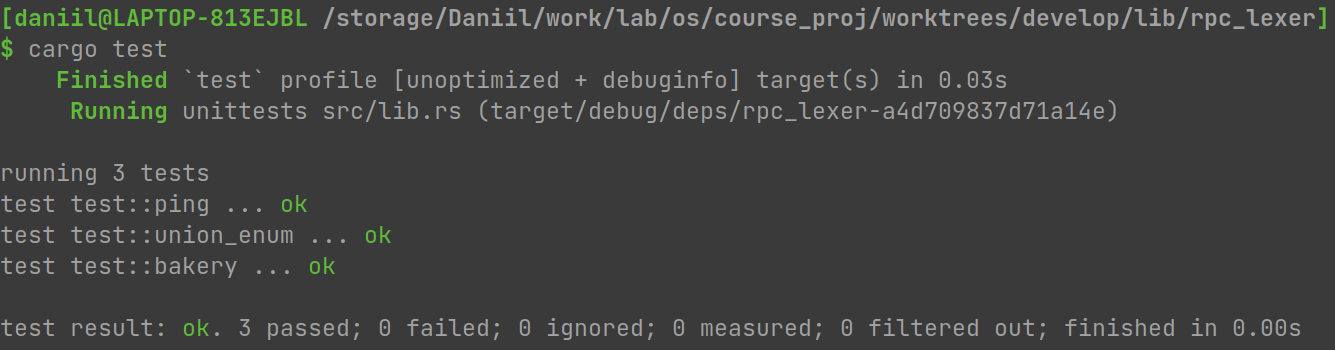
\includegraphics[width=\textwidth]{test_lexer.png}
    \caption{Тестирование лексического анализатора}
    \label{fig:test_lexer}
\end{figure}
\vfill

\clearpage

\begin{table}[htb!]
    \centering
    \begin{threeparttable}
        \caption{Тестирование синтаксического анализатора}
\begin{tabular}{|r|l|l|}
\hline
\multicolumn{1}{|c|}{№} & \multicolumn{1}{c|}{Исходные данные}                                            & \multicolumn{1}{c|}{Ожидаемый результат}                                                                                                                                                                                                                                                                       \\ \hline
1                       & \begin{tabular}[c]{@{}l@{}}Ping программа\\ изстандарта\end{tabular}            & \begin{tabular}[c]{@{}l@{}}Определенией программы PING\_PROGR,\\ содержащее 2 верcии: PING\_VERS\_PINGBACK,\\ состоящей из двух процедур PINGPROC\_NULL\\ и PINGPROC\_PINGBACK;\\ PING\_VERS\_PINGBACK, состоящей из одной\\ процедуры PINGPROC\_NULL, а также\\ определение константы PING\_VERS\end{tabular} \\ \hline
2                       & \begin{tabular}[c]{@{}l@{}}Bakery из курса\\ операционных\\ систем\end{tabular} & \begin{tabular}[c]{@{}l@{}}Определение констант, определение структуры\\ BAKERY,определение программы\\ BAKERY\_PROG с версией BAKERY\_VER и\\ процедурой BACKERY\_PROC\end{tabular}                                                                                                                           \\ \hline
3                       & \begin{tabular}[c]{@{}l@{}}Разбор\\ неиспользованных\\ типов enum\end{tabular}  & Определение enum                                                                                                                                                                                                                                                                                               \\ \hline
\end{tabular}
        \label{tbl:test_parser}
    \end{threeparttable}
\end{table}

\begin{figure}[!h]
    \centering
    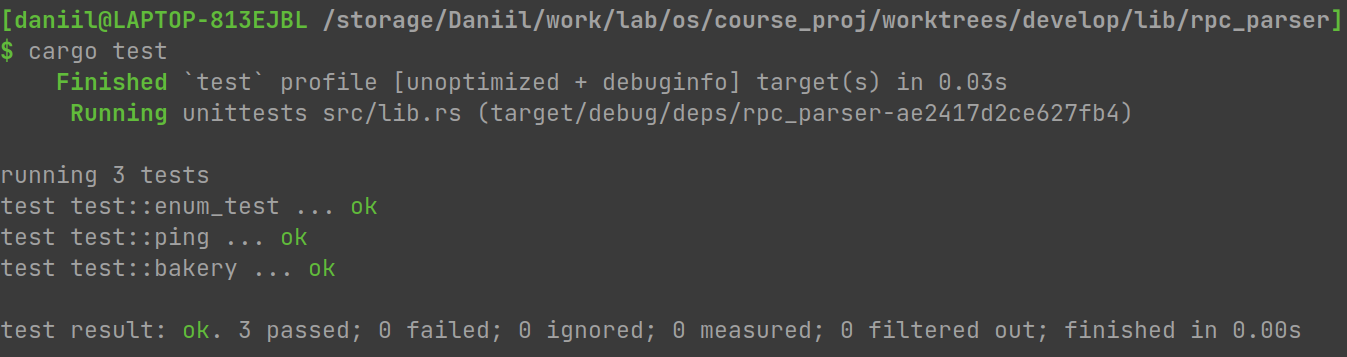
\includegraphics[width=\textwidth]{test_parser.png}
    \caption{Тестирование синтаксического анализатора}
    \label{fig:test_parser}
\end{figure}

\subsection*{Вывод}

В данном разделе были рассмотрены: структура разрабатываемого приложения и
генерируемых модулей ядра, средства и детали реализации программного продукта.

